\section{Experiments}\label{s:exp}
Next, we present experimental results that suggest two main conclusions: (1) as a single framework, \sys can achieve parity in terms of accuracy with state-of-the-art approaches to a variety of different problems ranging from integrity constraint satisfaction, statistical data cleaning, and also data cleaning for machine learning, (2) while the serial implementation of \sys can be much slower than the competitor specialized frameworks, \sys can be efficiently distributed to significantly reduce the gap.

\begin{figure}
    \centering
    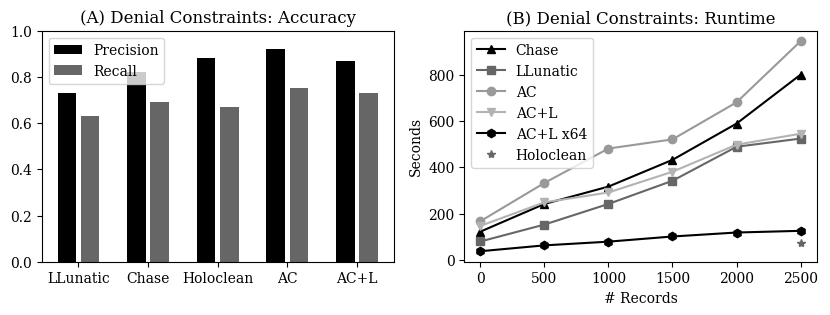
\includegraphics[width=\columnwidth]{exp/exp1.png}
    \caption{We compare \sys to alternative denial constraint systems on a dataset of flight arrival and departure times scraped from a variety of different sources. AC denotes \sys without any learned pruning and AC+L denotes \sys with pruning.
    \sys matches the accuracy of these systems and can be parallelized to match the runtime of these systems as well. Learning actually allows \sys to scale sub-linearly, i.e., as it sees more data it learns more precise pruning rules.\label{exp1a}}
\end{figure}

\subsection{Comparisons}
First, we compare \sys to a number of different baselines. To set expectations, \sys is a more general framework and we illustrate that it can match the accuracy of many more specialized frameworks. It is however slower in terms of runtime on certain problems. The goal of this section is to illustrate this tradeoff.

\subsubsection{Denial Constraints}
Several data cleaning systems use Denial Constraints for constraint specification. 
While \sys does not enforce integrity constraints, we can create a data quality objective function that quantifies the number of unsatisfied constraints.
This will search over a set of transformations that maximally satisfy these constraints.

\vspace{0.5em}\noindent\textbf{Flight Dataset: } The flight dataset contains arrival time, departure time, and gate information aggregated from 3 airline websites (AA, UA, Continental),
8 airport websites (such as SFO, DEN), and 27 third-party
websites.
There are 1200 flights departing from or arriving at the hub airports of the three airlines) from each source.
The data cleaning problem is to reconcile the differences between each sources.
Each flight has a unique flight identifier that is consistent across the websites.
Formally, we can model the reconciliation problem as functional dependency between the flight id and the arrival time, departure time, gate information.
This enforces that after resolution there will be a single canonical version of those values.

\vspace{0.5em}\noindent\textbf{Baselines: } We compare to two baselines: (1) Llunatic a denial constraint-based data cleaning systems~\cite{DBLP:conf/sigmod/DallachiesaEEEIOT13}, which is a C++ system implemented on Postgres SQL and (2) a restricted chase algorithm as in ~\cite{benedikt2017benchmarking} implemented in Python. 
We include (2) as a baseline because in experiments used in recent work, the majority of denial constraints were actually functional dependencies, and can be resolved using fixed-point iteration.
We also present numbers for comparison from a recently published system called Holoclean~\cite{rekatsinas2017holoclean} on the same datasets, but did not run the experiment ourselves.

\vspace{0.5em}\noindent\textbf{Results: } Figure \ref{exp1a} plots the results of this experiment. Figure \ref{exp1a}a shows the precision and recall of the various approaches w.r.t a gold-standard ground truth. \sys matches the accuracy of the other denial constraint based systems. Figure \ref{exp1a}b illustrates the runtime. While \sys without any learning is quite slow compared to the alternatives, learning can speed up the cleaning process significantly.
In fact, the results suggest that the scaling is \emph{sublinear}, where as the system sees more data it becomes more effective at pruning bad search branches.
For reference, we additionally include results parallelizing \sys on a 64 core machine with 64 search threads. This roughly matches the performance reported by Holoclean. 


\vspace{0.5em}\noindent\textbf{Other Datasets: } We also evaluated \sys on three  other datasets:
\begin{enumerate}
    \item The FEC provides a dataset of election contributions of 6,410,678 records with 18 numerical, categorical and string valued attributes. This dataset records the contribution with various demographic information about the contributors including name, address, and occuption.
    In this dataset, we enforced functional dependency relationships between city and zipcodes. We also matched the occupation of the contributors to a code book of popular occupations. This was posed as a quality function that was 1 only if the cell belonged to the code book and 0 otherwise, and there was an additive penalty on the edit distance between the change and the previous value.   
    \item The Malasakit dataset contains survey responses on disaster preparedness from the Philippines with 15 numerical and categorical attributes. In this dataset, we removed numerical outliers and pruned test data from the dataset. 
    \item The Physican dataset from  Medicare.gov contains information on physicians from the United States. There are a number of inconsistencies such as  spelling errors in the city names, zip code formatting, other organization name inconsistencies.
\end{enumerate}

The results are presented below with precision, recall, and a single-threaded runtime.
\begin{table}[ht]
\footnotesize
\centering
\begin{tabular}{|l|r|r|r|r|r|r|r|}
\hline
 & \#rows & \#cols & Pre & Rec & Runtime (s) \\
\hline
\hline
FEC	&6410678&18&0.94&	0.68&	18270s\\
\hline
Malasakit &1493& 15& 1.0 & 0.85& 1404s\\
\hline
Physican	&37465&10&1.0&0.84& 11761s\\
\hline
\end{tabular}
\end{table}

\begin{figure}
    \centering
    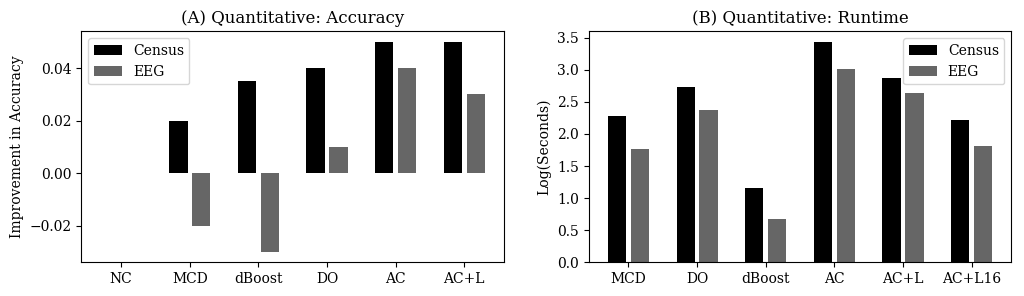
\includegraphics[width=\columnwidth]{exp/exp2.png}
    \caption{We evaluate \sys on a quantitative data cleaning task by cleaning a dataset prior to training a random forest classifier model. The system is allowed to clip outliers or set them to a default value. NC denotes no cleaning, MCD denotes using a Minimum Covariance Determinant approach to remove statistical outliers, DO denotes using \sys with only setting defaul values, and AC denotes \sys (+L with learning +L16 with learning and parallelized over 16 threads). (A) plots the accuracy of this classifier and (B) plots the run time. \label{exp2a}}
\end{figure}

\subsubsection{Quantitative Data Cleaning}
In this experiment, we consider handling numerical outliers in ML datasets.
In many machine learning settings, cleanly labeled test data is often available (e.g., the results of following a sales lead). 
Labels often represent directly observed phenomena making them relatively clean, while features are often weaker signals integrated from multiple disparate sources and subject to error and frequent change.
This allows us to define a quality function in terms of the model's predictive accuracy--the data cleaning being a means to improving that predictive accuracy.

\vspace{0.5em}\noindent\textbf{USCensus: } This dataset contains US Census records for adults and the goal is to predict  whether the adult earns more than $50,000$ dollars. It contains 32,561 records with 15 numerical and categorical attributes. This dataset contained a significant number of missing values coded as 999999.

\vspace{0.5em}\noindent\textbf{EEG: } This is a dataset of EEG recordings. 
The training data is organized into ten minute EEG clips labeled "Preictal" for pre-seizure data segments, or "Interictal" for non-seizure data segments. 
There are 2406 records each of which is a variable-length time-series of 16 attributes. We featurize this dataset into records of 32 attributes--the mean and variance over the length of the time-series. 
This dataset primarily contains numerical outliers, the clips have spurious readings.

\vspace{0.5em}
We defined a prediction task on each of these datasets. We trained a \textsf{sklearn} Random Forest classifier to predict the labels. The training procedure uses a set of standard featurizers (hot-one encoding for categorical data, bag-of-words for string data, numerical data as is) in a similar fashion as~\cite{gokhale2014corleone}. The quality function for \sys is 0 for each record that is incorrectly predicted by the model, 1 for each record that is correctly predicted by the model.

\sys is allowed to search through modifications to the records to try to make the prediction correct. We focused on transformations to numerical columns. Allowed data transformations are:
\[
\textsf{clip\_above}(attr, threshold), 
\]
which sets all values in $R[attr]$ above the threshold to threshold.
\[
\textsf{clip\_below}(attr, threshold), 
\]
which sets all values below threshold to threshold.
\[
\textsf{set\_default}(attr, value), 
\]
which sets all values in $R[attr]$ equal to value to the mean value.

\vspace{0.5em}\noindent\textbf{Baselines: } For this experiment, we defined a 20\% held-out test dataset. We apply the search on the 80\% of the training data, and apply the discovered transformations before predictions on the 20\% held-out set. 
We compare to the following baselines: (No Cleaning) there is no modification to the data before prediction, (Minimum Covariance Determinant) we apply the MCD, the outlier detection algorithm in ~\cite{bailis2016macrobase}, and it sets all detected outliers to the mean value, (dBoost) we use the partitioned histogram technique in dBoost~\cite{mariet2016outlier}, and (Default Only) we run \sys where the only operation is setting the mean value. 

\vspace{0.5em}\noindent\textbf{Results: } Figure \ref{exp2a} plots the results of the experiments. Without cleaning the classifier gets an accuracy of 82\% on the census dataset and 79\% on the EEG dataset. The MCD approach improves the classifer accuracy in the census dataset. This is because the majority of the outliers are very far from the mean, and MCD is an effective approach to identifying them. These outliers correspond to missing values so setting their value to the default mean is a sensible fix.
In the other dataset, EEG, the default mean fix is not always the best repair for outlier data. 
We found that clipping the value based on a threshold lead to the best classifier accuracy.
We came to this conclusion by running \sys with only the default value transformations and observed a similar pattern. 
By searching through the best transformations, \sys allows us to automatically make this decision.
The quality function for both datasets is the same but \sys finds very different transformation rules.

Of course, \sys is slower than the alternatives. 
Without any optimizations, \sys is nearly 10x slower than MCD.
But with learning, this gap is reduced to a factory of 4.
Furthermore, if we parallelize on 16 threads, we match the the runtime of MCD.
The runtime of the specialized outlier detection system, dBoost, is much faster and cannot be matched by \sys.

\begin{figure}
    \centering
    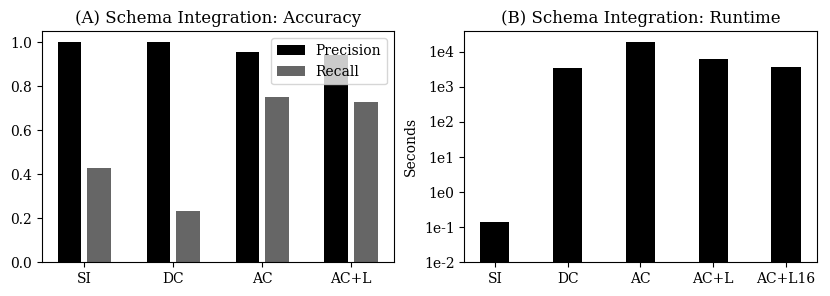
\includegraphics[width=\columnwidth]{exp/exp3.png}
    \caption{We evaluate \sys on a schema integration task from 55 different sources. There is a further data cleaning problem, where we would like to reconcile the values from different sources.
    (SI) Schema Integration only, where we use string similarity metrics to match the attribute names, (DC) Data cleaning only enforces FDs on those names that are already consistent, and  (AC) denotes \sys (+L with learning +L16 with learning and parallelized over 16 threads). \label{exp3a}}
\end{figure}

\subsubsection{Schema Integration}
In the next experiment, we consider a schema integration problem. This dataset considers data for 1000 ticker symbols from 55 sources that covers key trading metrics for every trading day in a month.
The challenge is to integrate the schema of these different sources. For example,
in one source the closing price is denoted by 'Prev. Close' and in another it is 'Previous Close'.
Once the schema is consistent, there is a further data cleaning problem, where we would like to reconcile the values from different sources. This can be achieved with a similar functional dependency relationship as described for the flight datasets.

\vspace{0.5em}\noindent\textbf{Baselines: } We consider the following baselines: (SI) Schema Integration only, where we use string similarity metrics to match the attribute names, (DC) Data cleaning only, we treat schema names as consistent and enforce the same functional dependencies with a restricted chase.

\vspace{0.5em}\noindent\textbf{Results: } Figure \ref{exp3a} plots the results of the experiment. If we apply schema integration only or only data cleaning there is a very high precision but poor recall. \sys can be used to perform both tasks and shows that we can improve the recall number significantly.
Furthermore, results suggest that we can run \sys at a competitive speed with parallelization over 16 threads.

 \begin{figure*}[ht]
\centering
 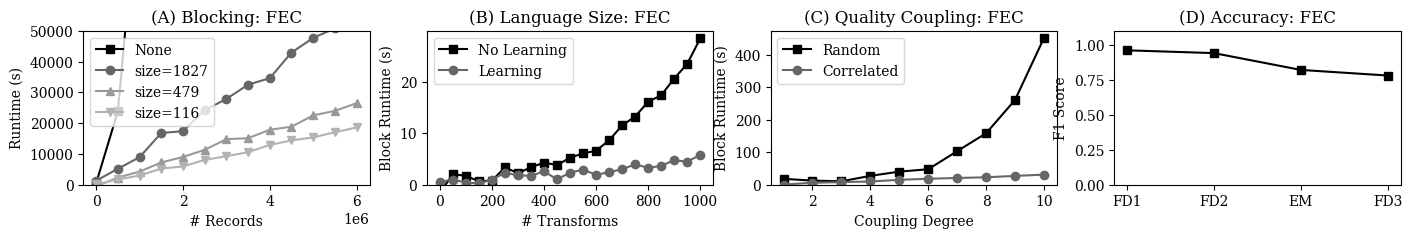
\includegraphics[width=\textwidth]{exp/exp4.png}
 \caption{(A) illustrates how the performance of \sys is affected block size, larger blocks require a longer search time, (B) shows how the search time scales as a function of the support of the transformation language, and learning can significantly reduce this time, (C) quality functions that have unpredictable couplings between multiple records together are harder to optimize, (D) \sys can handle compositions of multiple error types.
 \label{fig:microbenchmarks}}
\end{figure*}

\subsection{Properties of \sys}
In the next set of experiments, we evaluate key parameters that affect the performance of \sys.

\subsubsection{Key Variables}
First, we evaluate which parameters affect the difficulty of the search problem. We start with the FEC dataset described in the previous experiments. 

\vspace{0.5em}\noindent \textbf{Blocking: } Partitioning the dataset into smaller pieces effectively reduces the search horizon. For example, consider a dataset of 1000 records where each record requires an independent transformation. Rather than solving a search problem of depth 1000, we can solve 1000 search problems of depth 1.
The maximum granularity of blocks depends on the nature of the transformations and quality functions.
Currently, these blocks are set by the user in the form of predicates that partition the dataset.
Figure \ref{fig:microbenchmarks}a illustrates how the performance of \sys is affected block size. We partition the FEC dataset on three different attributes each with a different blocksize. The smaller the blocks the better the algorithm scales with the data. Without blocking, on this dataset, the search is very impractical.

\vspace{0.5em}\noindent \textbf{Language: } The next experiment (Figure \ref{fig:microbenchmarks}b) shows how the search time within a block scales as a function of the support of the transformation language. The more transformations there are, the higher the branching factor of the search problem. Without any optimizations, the search time is exponential in the language. But, once a pruning model is learned this time is significantly reduced.

\vspace{0.5em}\noindent \textbf{Quality Function Structure: } The nature of the quality function also affects the search time. Quality functions that couple multiple records together are harder to optimize (Figure \ref{fig:microbenchmarks}c).
Consider a function that requires that two different records must have the same attribute values.
More transformations have to be achieved in a particular sequence before an improvement in quality is observed. 
We selected between 1-10 records at random in each block and created a quality function that coupled these records together.
As the degree of coupling increases, the search time grows quite drastically.
We repeated the same experiment where now coupling is correlated with the data, i.e., we sort one of the attributes and couple ``nearby'' records.
\sys performs significantly better on this version of the task.
This is due to the learned pruning in \sys.
Sorting the attributes introduces a systematic correlation in the quality function.
\sys quickly learns a model which learns this correlation and uses that to prune the search space.

To illustrate how the structure of the quality function affects accuracy, we incrementally make the FEC data cleaning problem more difficult.
We first start with a single FD, then add another, then add rules to match entities, and then another FD.
The quality function used is a sum of the quality functions for each of the constraints.
As the quality function considers more and more constraints, it becomes harder to optimize.

 \begin{figure*}[ht]
\centering
 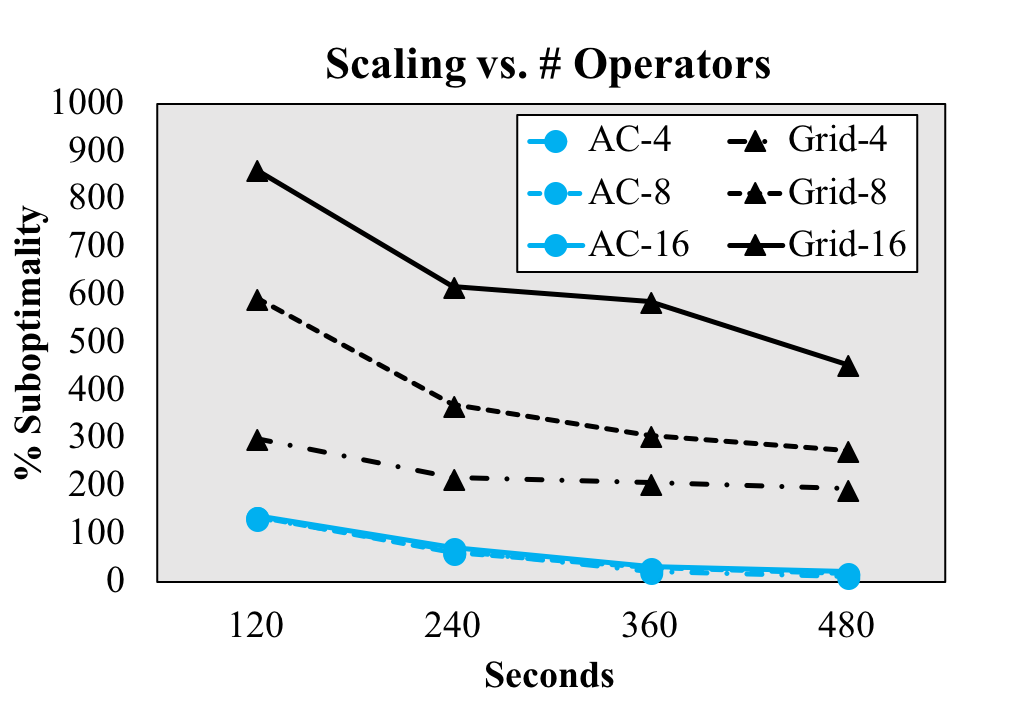
\includegraphics[width=\textwidth]{exp/exp5.png}
 \caption{ (A) We inject noise into the quality function to simulate a ``mis-specified'' objective and plot the F1 accuracy of \sys for different settings of the edit penalty, (B-C) overly specific rules may not apply to future data, and overly general rules, might introduce unwanted side-effects.
 \label{fig:sensitivity}}
\end{figure*}

\subsubsection{Generalization and Sensitivity}
There are some interesting properties that are specific to \sys with regards to sensitivity and generalization to unseen data. Figure \ref{fig:sensitivity}A plots the F1-score of \sys on the FEC dataset. We inject noise into the quality function to simulate a ``mis-specified'' objective. Predictably, the F1 score rapidly degrades as more noise is injected.
However, one can mitigate the effects of mis-specification by adding a penalty to the quality function that penalizes edits.
As the edit cost is increased, the baseline performance (for no noise) decreases, but the result is more robust to the noise injected.

Figure \ref{fig:sensitivity}B-C illustrates another interesting aspect of \sys, namely, a property akin to overfitting in machine learning.
We parametrized the transformation language with single attribute, double attribute, and triple attribute predicates.
Then, we applied \sys to sample of data.
We measured the ``in-sample error'' Figure \ref{fig:sensitivity}C, which is the F1 score with records inside the sample, and the ``out-of-sample'' error which is the F1 score on unseen records.
The more expressive two attribute predicates are most accurate on the in-sample metric, however, we not as accurate as the single attribute predicates on the out-of-sample metric.
The three sample predicates were very computationally expensive to search so the results are less reliable.
This result highlights an important point overly specific rules may not apply to future data, and overly general rules, might introduce unwanted side-effects.


\subsection{Algorithm Properties}
Finally, Figure \ref{fig:opt} illustrates the scaling properties of \sys. We run all of our experiments on a cluster of 4 mx.large EC2 instances. We compare three baseline implementations: (No opt.) a vanilla best-first search, (Cache) best-first search + materialization, (Cache+Comm) best-first search and reducing the communication with the algorithm described in the paper. 
Figure \ref{fig:opt}A shows how the run time on the FEC dataset varies as a function of the number of worker threads on the cluster.
With no optimizations and single threaded, the runtime is 4432 seconds.
If we use the materialization strategy described in the paper, we can reduce this runtime by a factor of 10 (432 seconds) even on a single thread.
As we scale out, we can further reduce this runtime.
We see that the Cache+Comm strategy scales better (67 seconds for 64 workers) than the naive Cache only strategy (137 seconds for 64 workers).
Interestingly enough, in relative terms, the vanilla best-first search strategy scales the best.
This is because with no materialization the only communication is the description of which transformations to expand.
However, it is slower by a factor of 10 in absolute numbers.

Figure \ref{fig:opt}B illustrates the effect of learning a search heuristic. As more blocks are cleaned, the system trains a classifier to prune implausible transformations in the future.
This means that the search time spent on each block is greatly reduced (75\%). 
Figure \ref{fig:opt}C shows that the best-first search is really the most practical algorithm in this setting, running order of magnitudes faster than a naive BFS or DFS.

 \begin{figure*}[ht]
\centering
 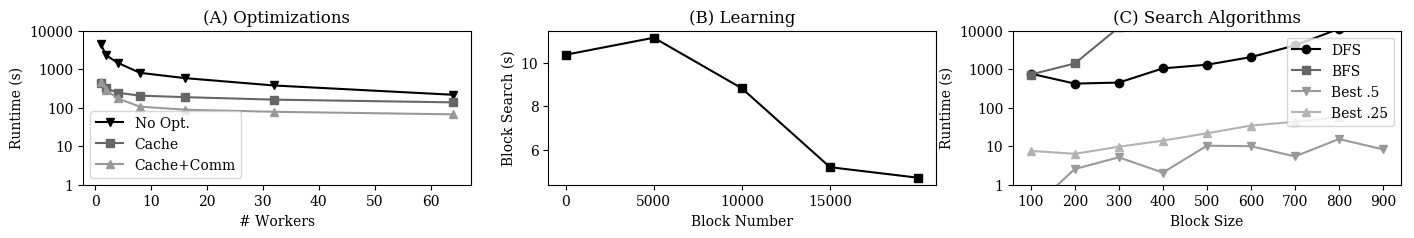
\includegraphics[width=\textwidth]{exp/exp6.png}
 \caption{(A) We compare three baseline implementations for scalability: (No opt.) a vanilla best-first search, (Cache) best-first search + materialization, (Cache+Comm) best-first search and reducing the communication with the algorithm described in the paper. (B) illustrates the effect of learning a search heuristic. (C) best-first search is much more effective than a BFS or DFS search.
 \label{fig:opt}}
\end{figure*}

